\documentclass[12pt, a4paper]{article}

\usepackage{amssymb}
\usepackage{multicol}
\usepackage{enumerate}
\usepackage[top=5em, bottom=5em, left=5em, right=5em]{geometry}
\usepackage{listings}
\usepackage{tikz}
\usetikzlibrary{positioning}

\setlength\parskip{1em}
\setlength\parindent{0em}

\title{Assignment 12}

\author{Hendrik Werner s4549775}

\begin{document}
\maketitle

This was done in collaboration with Constantin Blach (s4329872).

\section{} %1

\begin{enumerate}
	\item $T = \emptyset$
	\item Find the next house $h$ not covered by any tower. \label{sec1:find_house}
	\item \begin{itemize}
		\item If $h$ is found place a new tower $t = h.position + 4$. $T = T \cup \{t\}$
		\item else return $T$
	\end{itemize}
	\item Go to step \ref{sec1:find_house}
\end{enumerate}

Where $h.position$ indicates the position of house $h$ in miles from the start of the country road.

After using this algorithm, $T$ contains the positions where we need to place towers to cover all houses along the road.

\paragraph{Correctness}
For every new house $h$ we find at step \ref{sec1:find_house} we must place a cell tower that covers this house because we need to cover all houses. We place it the farthest away from this house as to still cover $h$. This ensures that we cover not only $h$ but as many other houses as possible because we place is as far along the road as possible at $h.position + 4$ while still covering $h$.

\paragraph{Time Complexity}
We need to visit every house once and perform $O(1)$ work there. The time complexity is $O(|H|)$ where $H$ is s list of houses ordered by their distance from the start of the road.

\section{} %2

\begin{itemize}
	\item The queue consists of tuples of edges and their weight.
	\item Thick edges were added to the minimum spanning tree.
	\item Blue edges were added to the spanning tree at this step.
	\item Gray vertices have been reached by the spanning tree.
\end{itemize}

Initial state:

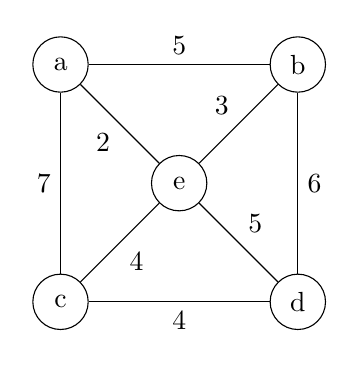
\begin{tikzpicture}[
	baseline=(A.north)
	,n/.style={draw, circle, minimum width=2em}
	,recently/.style={blue}
	,added/.style={line width=.2em}
]
	\node[n] (E) {e};
	\node[n, above left=of E] (A) {a};
	\node[n, above right=of E] (B) {b};
	\node[n, below left=of E] (C) {c};
	\node[n, below right=of E] (D) {d};

	\path (A) edge node [auto] {5} (B);
	\draw (B) edge node [auto] {6} (D);
	\draw (C) edge node [auto] {7} (A);
	\draw (D) edge node [auto] {4} (C);
	\draw (E) edge node [auto] {2} (A);
	\draw (E) edge node [auto] {3} (B);
	\draw (E) edge node [auto] {4} (C);
	\draw (E) edge node [auto] {5} (D);
\end{tikzpicture}

Queue: \begin{enumerate}
	\item $(\{e, a\}, 2)$
	\item $(\{e, b\}, 3)$
	\item $(\{e, c\}, 4)$
	\item $(\{d, c\}, 4)$
	\item $(\{e, d\}, 5)$
	\item $(\{a, b\}, 5)$
	\item $(\{b, d\}, 6)$
	\item $(\{a, c\}, 7)$
\end{enumerate}

\begin{enumerate}
	\item 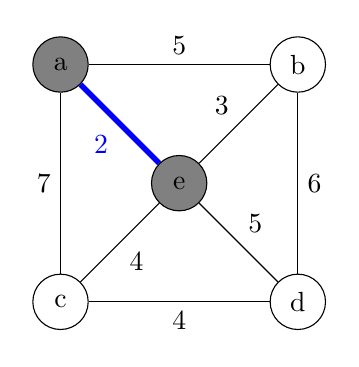
\begin{tikzpicture}[
		baseline=(A.north)
		,n/.style={draw, circle, minimum width=2em}
		,reached/.style={fill=gray}
		,recently/.style={blue}
		,added/.style={line width=.2em}
	]
		\node[n, reached] (E) {e};
		\node[n, reached, above left=of E] (A) {a};
		\node[n, above right=of E] (B) {b};
		\node[n, below left=of E] (C) {c};
		\node[n, below right=of E] (D) {d};

		\path (A) edge node [auto] {5} (B);
		\draw (B) edge node [auto] {6} (D);
		\draw (C) edge node [auto] {7} (A);
		\draw (D) edge node [auto] {4} (C);
		\draw[added, recently] (E) edge node [auto] {2} (A);
		\draw (E) edge node [auto] {3} (B);
		\draw (E) edge node [auto] {4} (C);
		\draw (E) edge node [auto] {5} (D);
	\end{tikzpicture}

	Queue: \begin{enumerate}
		\item $(\{e, b\}, 3)$
		\item $(\{e, c\}, 4)$
		\item $(\{d, c\}, 4)$
		\item $(\{e, d\}, 5)$
		\item $(\{a, b\}, 5)$
		\item $(\{b, d\}, 6)$
		\item $(\{a, c\}, 7)$
	\end{enumerate}
	\item 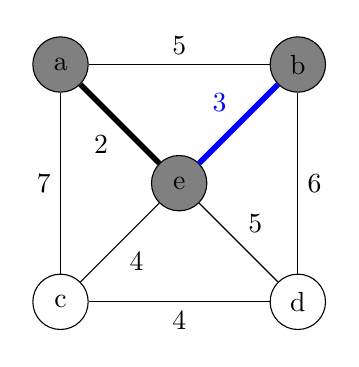
\begin{tikzpicture}[
		baseline=(A.north)
		,n/.style={draw, circle, minimum width=2em}
		,reached/.style={fill=gray}
		,recently/.style={blue}
		,added/.style={line width=.2em}
	]
		\node[n, reached] (E) {e};
		\node[n, reached, above left=of E] (A) {a};
		\node[n, reached, above right=of E] (B) {b};
		\node[n, below left=of E] (C) {c};
		\node[n, below right=of E] (D) {d};

		\path (A) edge node [auto] {5} (B);
		\draw (B) edge node [auto] {6} (D);
		\draw (C) edge node [auto] {7} (A);
		\draw (D) edge node [auto] {4} (C);
		\draw[added] (E) edge node [auto] {2} (A);
		\draw[added, recently] (E) edge node [auto] {3} (B);
		\draw (E) edge node [auto] {4} (C);
		\draw (E) edge node [auto] {5} (D);
	\end{tikzpicture}

	Queue: \begin{enumerate}
		\item $(\{e, c\}, 4)$
		\item $(\{d, c\}, 4)$
		\item $(\{e, d\}, 5)$
		\item $(\{a, b\}, 5)$
		\item $(\{b, d\}, 6)$
		\item $(\{a, c\}, 7)$
	\end{enumerate}
	\item 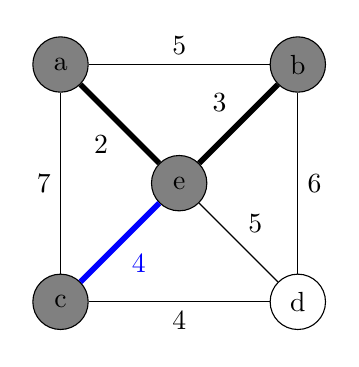
\begin{tikzpicture}[
		baseline=(A.north)
		,n/.style={draw, circle, minimum width=2em}
		,reached/.style={fill=gray}
		,recently/.style={blue}
		,added/.style={line width=.2em}
	]
		\node[n, reached] (E) {e};
		\node[n, reached, above left=of E] (A) {a};
		\node[n, reached, above right=of E] (B) {b};
		\node[n, reached, below left=of E] (C) {c};
		\node[n, below right=of E] (D) {d};

		\path (A) edge node [auto] {5} (B);
		\draw (B) edge node [auto] {6} (D);
		\draw (C) edge node [auto] {7} (A);
		\draw (D) edge node [auto] {4} (C);
		\draw[added] (E) edge node [auto] {2} (A);
		\draw[added] (E) edge node [auto] {3} (B);
		\draw[added, recently] (E) edge node [auto] {4} (C);
		\draw (E) edge node [auto] {5} (D);
	\end{tikzpicture}

	Queue: \begin{enumerate}
		\item $(\{d, c\}, 4)$
		\item $(\{e, d\}, 5)$
		\item $(\{a, b\}, 5)$
		\item $(\{b, d\}, 6)$
		\item $(\{a, c\}, 7)$
	\end{enumerate}
	\item 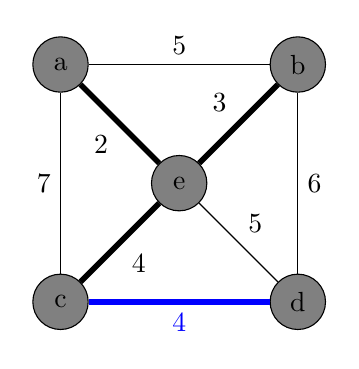
\begin{tikzpicture}[
		baseline=(A.north)
		,n/.style={draw, circle, minimum width=2em}
		,reached/.style={fill=gray}
		,recently/.style={blue}
		,added/.style={line width=.2em}
	]
		\node[n, reached] (E) {e};
		\node[n, reached, above left=of E] (A) {a};
		\node[n, reached, above right=of E] (B) {b};
		\node[n, reached, below left=of E] (C) {c};
		\node[n, reached, below right=of E] (D) {d};

		\path (A) edge node [auto] {5} (B);
		\draw (B) edge node [auto] {6} (D);
		\draw (C) edge node [auto] {7} (A);
		\draw[added, recently] (D) edge node [auto] {4} (C);
		\draw[added] (E) edge node [auto] {2} (A);
		\draw[added] (E) edge node [auto] {3} (B);
		\draw[added] (E) edge node [auto] {4} (C);
		\draw (E) edge node [auto] {5} (D);
	\end{tikzpicture}

	Queue: \begin{enumerate}
		\item $(\{e, d\}, 5)$
		\item $(\{a, b\}, 5)$
		\item $(\{b, d\}, 6)$
		\item $(\{a, c\}, 7)$
	\end{enumerate}
\end{enumerate}

Minimum spanning tree:
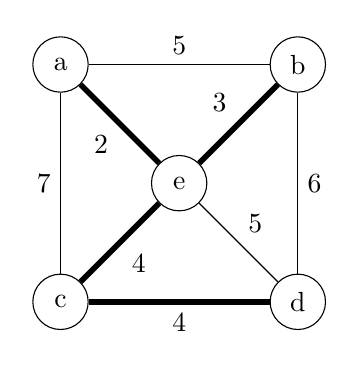
\begin{tikzpicture}[
		baseline=(A.north)
		,n/.style={draw, circle, minimum width=2em}
		,reached/.style={fill=gray}
		,recently/.style={blue}
		,added/.style={line width=.2em}
	]
		\node[n] (E) {e};
		\node[n, above left=of E] (A) {a};
		\node[n, above right=of E] (B) {b};
		\node[n, below left=of E] (C) {c};
		\node[n, below right=of E] (D) {d};

		\path (A) edge node [auto] {5} (B);
		\draw (B) edge node [auto] {6} (D);
		\draw (C) edge node [auto] {7} (A);
		\draw[added] (D) edge node [auto] {4} (C);
		\draw[added] (E) edge node [auto] {2} (A);
		\draw[added] (E) edge node [auto] {3} (B);
		\draw[added] (E) edge node [auto] {4} (C);
		\draw (E) edge node [auto] {5} (D);
	\end{tikzpicture}

\section{} %3

Because we want to use as few rooms as possible and have no further restrictions about what to do with the activities (for example, a maximum total length of the schedule), we cen just schedule all activities in the same room after each other. This is trivially correct and uses $0$ rooms if $S = \emptyset$ and $1$ room otherwise. The time complexity is obviously $O(1)$ since we just need to return what we got.

\section{} %4

\section{} %5

The first step is finding a minimum spanning tree $S$ in $G$, using Prim's algorithm.

Assume there is another minimum spanning tree. This means we can replace some edges by other edges that do not break the spanning tree and still have the same weight. For every edge $e \in S$ we already found however we cannot replace it with another edge $e' \not\in S$ because $e'$ cannot have the same weight as $e$ because all weights are unique and it cannot weigh less because then we would have picked it over $e$ in the first step with Prim's algorithm where we pick edges in order of their weight.

It follows that no edge in $S$ can be replaced while maintaining the minimum weight so $S$ must be the only possible minimum spanning tree.

\end{document}
